\section{Method}
\begin{figure*}[t]
    \centering
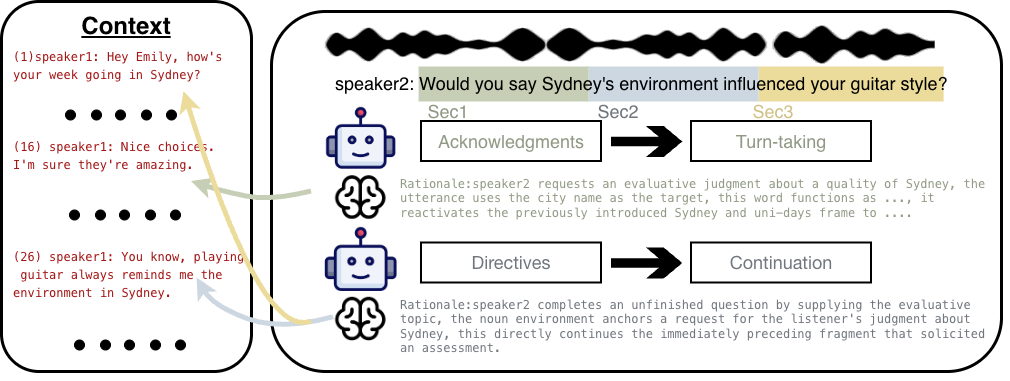
\includegraphics[width=0.9\linewidth]{fig/Method/pipeline_4.png}
\vspace{-5pt}
    \caption{{\bf Causal streaming pipeline for conversational behavior modeling.} At each 1~s tick, the model causally predicts hierarchical speech acts and generates an evidence-grounded rationale using a sliding-window Graph-of-Thoughts (GoT).}
    \label{pipeline}
\end{figure*}

As shown in Fig~\ref{pipeline}, our framework combines multi-level speech act perception with GoT reasoning to capture the perceptual pathway of human conversation. Our system performs online prediction at the per-second level. Each second, it outputs a two-level speech act and the corresponding rationale as explanation. The model is strictly causal and streaming (it can only access the current second and past audio information). We construct ConversationGoT-120h, a training dataset that includes high-quality dialogue content, synthetic audio, and human-verified rationale annotations, to train our framework. In addition, we train a multi-level, causal, and streaming perceiver to output perception results for per-second speech action. Finally, we use GoT to reason and generate high-quality rationale as an explanation.
\subsection{ConversationGoT-120h}
\paragraph{Motivation. } Existing full-duplex datasets primarily emphasize low-level acoustic dynamics (e.g., 20–40 ms frame-based events) or token-level modeling. We shift the focus to decision-level conversational behaviors paired with verifiable rationales, producing behavior decisions with controllable latency and auditable, checkable explanations. Therefore, we choose a 1s time step to output two-level speech acts (high/low) and rationale, balancing latency, annotation noise, and compute budget. Meanwhile, existing datasets often lack a unified annotation framework for multi-level speech act plus rationale, making it difficult to systematically model conversational behaviors. More critically, many works leverage the global structure of the full dialogue when annotating or generating labels, introducing a risk of causal leakage. To this end, we build ConversationGoT-120h: a training dataset covering 120 hours, with dialogue content closer to real scenarios, and providing two-level speech act and high-quality rationale, spanning diverse speaker identities, topics, acoustic conditions, and dialogue styles; and explicitly aligning the annotation and generation mechanisms with a strictly causal setting to minimize causal leakage. This dataset represents a novel step toward hierarchical behavior modeling in dialogue, facilitating the development of models that provide perceptually grounded explanations alongside standard label outputs.
% We believe this is one of the first datasets for hierarchical conversational behavior modeling, enabling models to learn not only to output labels, but also to output perceptually grounded explanations.
\paragraph{Speech Acts and Rationale.} 
Low speech acts include Backchannel, Interruption, Turn-taking, and Continuation. High speech acts include Constatives, Directives, Commissives, and Acknowledgments. All Speech Acts are generated under a causal constraint by design. See the Appendix for the formal definition. Rationale is an open-form reasoning text used to explain and justify the current conversation behavior, characterizing the finest-grained level of conversational behavior perception.

\paragraph{Generation.}Our dataset targets open domain chit-chat dialogues. To obtain dialogue text with diverse content, natural topic transitions, and rich character settings, we design a structured data generation pipeline: we first use a GPT-4o~\cite{openai2024gpt4ocard} to synthesize speaker identity information (such as interests, birthplace, education background, and family background); based on this, we generate 8–10 topics for each dialogue, and split them into interactive topics (jointly discussed by both sides) and expressive topics (primarily led by a single speaker). When generating each topic, we mask the full identity information and use only 1–2 traits for conditional generation to reduce repetition and improve content diversity. Then, given the identity information and topic sequence, we complete transitions between topics and generate the beginning and ending of the dialogue, making the overall dialogue more coherent.

To provide supervision signals consistent with a strictly causal setting, we model the dialogue second by second: we segment audio/text into consecutive 1s chunks, and generate hierarchical speech acts and rationale without relying on the global dialogue structure. Specifically, we first use a GPT-4o~\cite{openai2024gpt4ocard} to retrieve remote content anchor sentence(s) for the current second, and organize them from far to near into a topic thought chain; we then feed this topic chain together with the observable inputs of the current second into a reasoning GPT5~\cite{singh2025openaigpt5card}, so that it gradually derives the speech act (high/low) label for the current second, and we save the step by step reasoning process as the rationale annotation. Meanwhile, these saved anchors provide multi-hot supervision for Stage-1 selection. As a result, the dataset can supervise GoT to learn the reasoning chain required for decision making, rather than performing post hoc attribution analysis toward predefined labels. 

Finally, we synthesize audio: we collect 1,166 high quality reference voices from LibriSpeech \citep{panayotov2015librispeech}, and use CosyVoice2 \citep{du2024cosyvoice} to synthesize speech that is closer to real conversations and has more diverse prosody; we obtain 1,440 samples with an average duration of about 5 minutes, totaling about 120 hours of ConversationGoT-120h.

\subsection{Speech Acts Perceiver}
Our SA predictor is designed around two principles: realistic perception should be hierarchical, and the entire model must operate in a streaming, strictly causal setting. Prior work often treats speech act observation as a single level, one shot prediction event, overlooking human hierarchical perception of conversational events. Humans typically first perceive speech act at the utterance and turn level, and then, on this basis, predict the other speaker’s next concrete conversational action, which is the key to reliable perception. For example (Figure~\ref{pipeline}), at the 1 second in the figure, humans first identify from within utterance second information that a new turn is being initiated, namely that this segment is at the beginning of the sentence and uses a typical question initiating template. Meanwhile, combined with the historical context in which “Sydney” has been repeatedly introduced in earlier multiple turns and associated with “playing guitar”, humans further, at a fine grained level, judge its intent as a Directives “evaluation request”.

To characterize the relationship between high-level and low-level acts, we compute the empirical mean low-level distribution conditioned on each high-level act. Concretely, for each high-level category $h$, we estimate \begin{equation} \bar{p}(y \mid h)=\frac{1}{N_h}\sum_{i:\,h_i=h}\mathbb{I}[y_i=y], \end{equation} where $y$ denotes the low-level label, $N_h$ is the number of instances with high-level label $h$, and $\mathbb{I}$ is the indicator function. As shown in Table~\ref{tab:JSD_for_SA}, the conditional low-level distributions differ substantially across high-level categories; in particular, Acknowledgments assigns markedly higher mass to Backchannel than other high-level acts, indicating a distinct interaction pattern.
\begin{table}[t]
\centering
\caption{Conditional Distribution for SA}
\label{tab:JSD_for_SA}

{\fontsize{7.5}{9.5}\selectfont
\renewcommand{\arraystretch}{0.92} 
\setlength{\tabcolsep}{3pt}     

\begin{tabular}{@{}l|cccc@{}}
\toprule
cond. dist.($\uparrow$) & Continuation & Turn-taking & Interruption & Backchannel \\
\midrule
Constatives      & \textbf{0.5375} & 0.2280 & 0.1320 & 0.1025 \\
Directives       & \textbf{0.4903} & 0.2409 & 0.1619 & 0.1069 \\
Acknowledgments  & 0.2552 & 0.2325 & 0.1593 & \textbf{0.3530} \\
Commissives      & \textbf{0.4723} & 0.2620 & 0.1393 & 0.1264 \\
\bottomrule
\end{tabular}
}
\end{table}


\paragraph{Problem Definition.}
We formulate hierarchical sequential modeling as a strictly causal streaming hierarchical sequence, as a stepwise conditional classification problem, and further use an autoregressive factorization to express online prediction. The model takes as input a dialogue speech signal $X=\{x_t \mid t=1,\ldots,T\}$, represented as a time-series of length $T$.
% \begin{equation}
% X=\{x_t \mid t=1,\ldots,T\}.
% \end{equation}
For two-channel full-duplex recordings, we downmix the channels into a single-channel mono mixture using a per-sample linear combination, which preserves causality, and resample the signal to $f_s=16,\text{kHz}$.
 Let the number of samples in each 1-second block be
$N_{\text{block}} = f_s$, then the entire audio is partitioned into $N=\left\lceil T/N_{\text{block}} \right\rceil$ continuous, non-overlapping speech blocks $U=\{U_i\}_{i=1}^{N}$. The goal is to predict hierarchical speech acts at the segment level: a high-level label sequence
$Y^{H}=\{y_i^{H}\}_{i=1}^{N}$ and a low-level label sequence $Y^{L}=\{y_i^{L}\}_{i=1}^{N}$.
At step $i$, the output can only depend on the current and past inputs $U_{\le i}$ (or a restricted window thereof), and cannot access future blocks $U_{>i}$. Accordingly, we directly model a family of causal conditional distributions and write the joint conditional distribution as an autoregressive factorization:
\begin{equation}
p_\theta(Y^{H},Y^{L}\mid X)
=
\prod_{i=1}^{N}
p_\theta\!\left(y_i^{H},y_i^{L}\mid U_{\le i}\right).
\end{equation}
Using a causal decomposition (i.e., the low-level prediction is explicitly conditioned, in the causal sense, on the high-level information at the same time step), we obtain
\begin{equation}
p_\theta(Y^{H},Y^{L}\mid X)
=
\prod_{i=1}^{N}
p_\theta\!\left(y_i^{H}\mid U_{\le i}\right)\,
p_\theta\!\left(y_i^{L}\mid y_i^{H},U_{\le i}\right).
\end{equation}
\paragraph{Model Details.}
We propose a hierarchical speech modeling framework that combines complementary acoustic and semantic cues, and explicitly injects high-level context to guide low-level prediction. For each speech block $U_i$, we obtain frozen acoustic and semantic embeddings $(h_i^{B}, h_i^{E})$ and fuse them via element-wise gating:
\[
\lambda_i=\sigma(W_b h_i^{B}+W_e h_i^{E}),\quad
e_i=(1-\lambda_i)\odot h_i^{B}+\lambda_i\odot h_i^{E}.
\]
The fused representation is mapped to a shared latent space $\tilde z_i=g_{\text{shared}}(e_i)$. To capture hierarchical temporal dependencies, we use two causal Transformer decoders to produce high-level state $z_i^H=g_H(\tilde z_{\le i})$ and low-level state $z_i^L=g_L(\tilde z_{\le i})$.
% \[
% z_i^H=g_H(\tilde z_{\le i}),\qquad z_i^L=g_L(\tilde z_{\le i}).
% \]
We further realize high-level guidance for low-level prediction by modulating the low-level stream with FiLM parameters predicted from the high-level state:
\[
(\gamma_i,\eta_i)=g_{\text{FiLM}}(z_i^H),\quad
\tilde z_i^L=\gamma_i\odot z_i^L+\eta_i.
\]
Finally, task-specific heads output predictions for the high-level and low-level tasks. More detail is provided in appendix.

The training objective is defined as the sum of cross-entropy losses over all valid time steps
% \paragraph{Loss Function.}
% We adopt multi-task supervision, with the training objective defined as the sum of cross-entropy losses over all valid time steps:
\begin{equation}
\mathcal{L}=\sum_i \mathrm{CE}\!\left(y_i^{H},o_i^{H}\right)+\mathrm{CE}\!\left(y_i^{L},o_i^{L}\right).
\end{equation}


\subsection{Graph of Thought}
Our design targets strict latency budgets. Prior work often uses LLM reasoning verbatim as the explanation, but such reasoning incurs high and hard-to-control runtime latency. We therefore use LLM reasoning traces only as training supervision, so GoT can imitate the teacher’s intermediate evidence and decision path while generating rationales with minimal overhead and less post-hoc rationalization.

To make GoT closer to human online perception and inference, we draw on a key cognitive logic: humans often combine grammatical cues, semantic templates, and historical context chains to gradually form and verify hypotheses about conversational behavior. For example, at the 1 second in Figure \ref{pipeline}, humans first judge that a new turn is initiated based on the sentence-initial grammatical structure and the typical question semantic template triggered within that second. They then use the “Sydney + playing guitar” topic chain in the historical context for grounding, and finally categorize the intent as an “evaluation request” under Directives. Accordingly, we represent the input as a hierarchical sliding-window graph with sentence nodes and second-level nodes. A low-latency topic-chain selector retrieves relevant sentence nodes for the current second; we then add directed edges to form a pseudo-causal graph and feed it to the decoder to generate rationales.

\paragraph{Graph Definition.}
At each time step, we define the dialogue context within the sliding window as a dynamic graph, containing two types of nodes: second-level node and sentence node. For any second-level node $t$, its attributes include speaker identity $s_t$, the relative time position $t$ within the window, the transcript text segment $x_t$ of that second, the audio segment $a_t$ of that second, and the hierarchical speech-act input label $y_t$ of that second. For any sentence node $k$, its attributes include the relative time interval $[\tau_k^s,\tau_k^e)$ within the window,  speaker identity $s_k$, and the transcript text $X_k$ of that sentence.

Within the window, second-level nodes represent those seconds that still belong to an uncommitted sentence segment, while sentence nodes represent committed sentence segments. When a sentence segment becomes committed, all second-level nodes whose time positions fall within $[\tau_k^s,\tau_k^e)$ are conceptually folded into a single sentence node $k$, and are replaced by this sentence node in the graph. As the window moves forward, the current time step appends new second-level nodes, and sentence nodes earlier than the window range are removed; the graph always contains exactly the second-level nodes and sentence nodes whose time positions fall within the current window.

\paragraph{Problem Definition.}
We model second-by-second online conversational behavior explanation as a strictly causal streaming select-augmented generation problem. By providing a coarse-grained, low-overhead guiding signal, we steer the decoding model toward the desired distribution. The observable input is the observation $(o_t)$ within a strictly causal history window, from which we construct a query node $(q_t)$ and a candidate sentence-node set $(C_t)$. The first stage introduces a latent evidence-chain variable $(\pi_t \subseteq C_t)$. It provides a coarse-grained inference signal for subsequent generation, approximately characterizing which historical sentence-segment evidence the teacher LLM would rely on when reasoning about the current second. Thus we formalize selection as approximate inference of the latent posterior:
\[
\pi_t \sim p_\phi(\pi_t \mid o_t),
\]
where $(\pi_t)$ intended to the reachability of the teacher conditional likelihood. During data construction, reachability is approximated by the teacher-LLM retriever used to build the rationale. $\pi_t^\star$ denotes the retriever-selected anchor set. During training, we learn from the supervised signal $\pi_t^\star$. In inference, we obtain an anchor chain via a thresholding approximation:
\(\hat{\pi}_t = \arg\max_{\pi_t} p_\phi(\pi_t\mid o_t), \quad\)
In the second stage, on top of \((\hat{\pi}_t)\), we incorporate more nearby fine-grained information to construct the final decoding condition \((\xi_t)\):
\(\xi_t \triangleq \big(\hat{\pi}_t,\ R_t,\ P_t,\ q_t\big),\)
and autoregressively generate rationale in a strictly causal manner:
\[
p_\theta(y_t\mid o_t,\hat{\pi}_t, R_t, P_t) = \prod_{n=1}^{|y_t|} p_\theta\!\left(y_{t,n}\mid y_{t,<n},\ \xi_t\right).
\]
Intuitively, $(\hat{\pi}_t)$ provides a global topic chain, while $((R_t,P_t,q_t))$ provides local observable details; together they determine the final LLM-style reasoning text.
\paragraph{Model Details.}
Under streaming audio, we run online speaker tracking, streaming ASR, and a per-second SA predictor in parallel. Every 1s tick, we aggregate the incremental ASR words into a second text $S_\tau$, assign a speaker tag $p_\tau$ from the speaker posterior, and attach SA labels $(\ell_\tau^{h},\ell_\tau^{l})$ to create a second node $v_\tau^{\mathrm{sec}}$. Sentence nodes are committed online with a causal sentence buffer; their speaker is set by within-sentence majority vote, and subsequent second nodes reference the updated sentence\_id. All features use only past observations, satisfying strict causality.

For evidence selection at time $t$, we use the current second node as query $q_t:=v_t^{\mathrm{sec}}$ and collect completed sentence nodes in the causal window $[t\!-\!W,t)$ as candidates $C_t$. We encode $V_t=\{q_t\}\cup C_t$ with a fully-connected Graph Transformer to model query--candidate matching and candidate competition (de-redundancy). We add a relational bias only on query$\rightarrow$candidate attention to inject temporal/structural cues while keeping candidate--candidate interactions unbiased. The model outputs candidate scores $s_{t,j}$ and a query-dependent threshold $\tau_t$; we select all anchors with $s_{t,j}>\tau_t$ and sort them into an evidence chain.

Given the selected anchors $\hat{\mathcal A}_t$, we augment them with lightweight causal caches (recent committed sentences $R_t$ and within-sentence seconds $P_t$), then sort all nodes by time and connect only adjacent ones to form a past$\rightarrow$present chain. Rather than adding another graph network, we linearize this chain into a token sequence for a T5 encoder; the decoder then generates the current-second rationale under cross-attention, fusing coarse sentence-level and fine second-level evidence.
\paragraph{Loss Function.}
Selector Loss: For each sample $(\text{audio\_id},t)$, the selector outputs candidate sentence scores $s_{t,j}$ and a dynamic threshold $\tau_t$. Define threshold-aligned logits:
\[
\ell_{t,j}=\frac{s_{t,j}-\tau_t}{T}.
\]
Given multi-hot labels $y_{t,j}\in\{0,1\}$ and a candidate mask $m_{t,j}$, the loss of the Stage-1 selector is
\[
\mathcal{L}_{\mathrm{sel}}
=\mathcal{L}_{\mathrm{wbce}}
+\lambda_{\mathrm{count}}\mathcal{L}_{\mathrm{count}}
+\lambda_{\mathrm{rank}}\mathcal{L}_{\mathrm{rank}},
\]
where the weighted BCE (only on valid candidates) is
\[
\mathcal{L}_{\mathrm{wbce}}
=\frac{1}{\sum_j m_{t,j}}\sum_j m_{t,j}\,\mathrm{WBCEWithLogits}(\ell_{t,j},y_{t,j};\alpha),
\]
and we use two lightweight regularizers:
\[
\mathcal{L}_{\mathrm{count}}=\Big(\sum_j\sigma(\ell_{t,j})-\sum_j y_{t,j}\Big)^2
\]
to constrain the selected count,
\[
\mathcal{L}_{\mathrm{rank}}=\frac{1}{|P_t|}\sum_{j\in P_t}-\log\frac{e^{\ell_{t,j}}}{\sum_k e^{\ell_{t,k}}}
\]
to promote positive-sample ranking, where $P_t=\{j:m_{t,j}=1,y_{t,j}=1\}$.
Decoder (T5 per-second rationale) loss.
Given the tokenized input $\mathbf{x}_t$ (linearized causal evidence chain) and the target rationale tokens $\mathbf{y}_t=(y_{t,1},\ldots,y_{t,L})$, we train the T5 decoder with standard teacher-forced seq2seq negative log-likelihood:
\[
\mathcal{L}_{\mathrm{dec}}
=-\sum_{n=1}^{L}\log p_\theta\!\left(y_{t,n}\mid y_{t,<n},\mathbf{x}_t\right).
\]
